\documentclass{IEEEtran}
\usepackage{lettrine}
\usepackage{tabu}
\usepackage{longtable}
\usepackage{tabularx}
\usepackage{amsmath}
\usepackage{graphicx}

\begin{document}
	
\title{Survey of RDBMS vs. Graph Database Performance Using Time Series Data Manipulation}
\author{Paul Marquardt and Kristen Rollins 
\thanks{This project draft was submitted for a grade on March 17, 2019. The project was completed under the supervision of Dr. Daniel Engels at Southern Methodist University.} 
\thanks{The authors can be contacted by email: Paul Marquardt at pmarquardt@smu.edu and Kristen Rollins at kmrollins@smu.edu.}}

\maketitle

\begin{abstract}
Performance constitutes an important aspect of database management and application development. An interesting project consists of measuring the performance, data model differences, and capabilities between both a graphing database system and RDBMS. This project compares times series data with data manipulation to capture and measure DBMS internal and OS level metrics including CPU, RAM, and disk performance statistics. 
\end{abstract}

\begin{IEEEkeywords}
	databases, relational databases, MySQL, graph databases, Neo4j
\end{IEEEkeywords}


\section{Introduction}

\lettrine{I}{n} today’s world, there are nearly countless database systems that have been developed and are available to use for a given application. While there may be many accessible programs, we know that different types of database systems are more appropriate to use in some situations than others. One such application that we wanted to investigate is the storage and manipulation of time series data.  The two types of database systems we have aimed to compare in this domain are relational and graph DBMSs. Here we describe the specific time series application as well as the two types of database systems, in order to gain background information and context for the ultimate problem we have researched.   

\subsection{Stock Exchange Data and VIR}

In our research, we utilized data from three American stock exchanges. Those were the AMEX, NASDAQ, and NYSE exchanges, which are the three largest financial securities markets in the United States. Each company belonging to these markets is identified by a stock symbol, or ticker symbol. For all of these symbols, each day the attributes of high, low, open, close, and volume are recorded. Using this data, we are able to compute a calculation of interest known as a Volatility Index Rating. 

The Volatility Index Rating, or VIR, calculation can be made for each symbol for each day. This value is a relative measure of how volatile a company’s stocks are estimated to be on a given day, based on recent trading behavior. This gauge of volatility, when observed closely, can lead to useful insights and profitable trading strategies. Such profits are expected to occur when a company's stock value is observed to be increasing, while the symbol’s VIR is low or decreasing. As indicated in Fig. \ref{fig:vir_example}, in this situation it would be profitable for a trader to purchase stock in that company, as the value is expected to continue increasing in a non-volatile manner. 

\begin{figure}
	\centering
	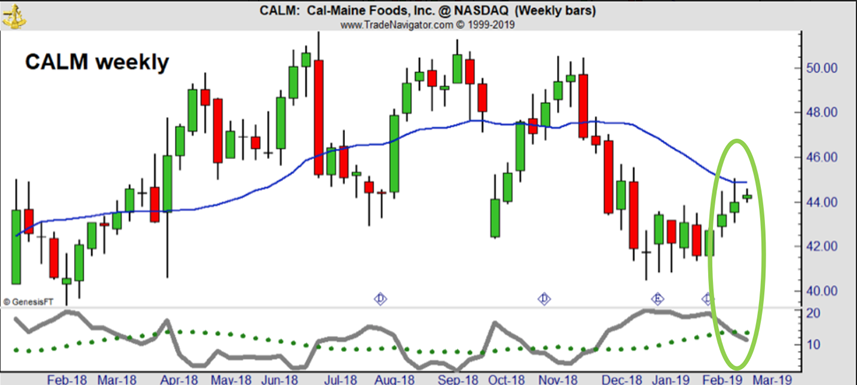
\includegraphics[width=3.5in]{Images/vir_example.png}
	\caption{VIR is shown by the grey line under the stock value fluctuation. The green oval indicates a profitable moment to purchase stock, as the stock value is increasing while the VIR is decreasing.}
	\label{fig:vir_example}
\end{figure}

The formula for VIR on a given day is computed using the symbol's data from the previous 22 days. The calculation is given in Equation \ref{eq:vir}. The resulting value is a percentage, as indicated by the factor of 100 in the equation. 

\begin{equation}
\text{VIR} = \frac{(\text{Highest Close} - \text{Current Low})}{\text{(Highest High)}} \cdot 100 \label{eq:vir}
\end{equation}

\subsection{Database Management Systems}

With the goal in mind of storing and manipulating stock exchange data, we must understand and utilize database management systems. Such systems work to let users create and maintain databases, while securely allowing appropriate access to users. Two opposing types of DBMSs are relational and graph databases. We chose these two families of database systems because of their stark differences yet wide-spread use. With these two systems we could store our stock data with differing schemas and strategies, in order to determine which is more appropriate for our application.

\subsubsection{Relational DBMS}

Relational database management systems serve many purposes for applications today. RDBMSs store data in a very structured, tabular format, and consist of rows or records as well as columns or attributes. Primary keys are used to uniquely identify records, and foreign keys enable relationships between tables. The specific relational DBMS we chose to perform our research with was MySQL. This RDBMS is open source and widely used for the needs of many applications.  

\subsubsection{Graph DBMS}

Graph database systems take a very different approach than do RDBMSs. Data are stored in nodes, which may have labels to categorize them. Graphs also consist of relationships, which can connect nodes in a certain direction, and properties, which can describe either nodes or relationships. A simple example is found in Fig. \ref{fig:graphdb_ex}. This representation of data can be very powerful and is able to serve the needs of a different class of applications. We chose Neo4j as our graph DBMS because it is open-source and the most popular graph database system.  

\begin{figure}
	\centering
	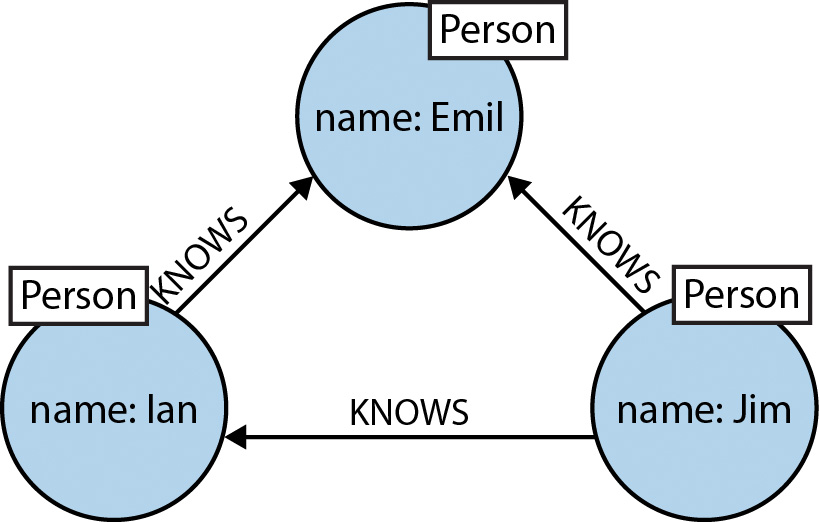
\includegraphics[width=3in]{Images/graphdb_simple_example.jpg}
	\caption{In this simple graph example, the blue circles represent nodes, each having the "Person" label. All of the nodes have a "name" property, seen inside each node. The lines between nodes indicate the "knows" relationship, with the arrow denoting the direction; e.g. Jim knows Ian, and Jim and Ian both know Emil.}
	\label{fig:graphdb_ex}
\end{figure} 

\subsection{Problem Statement}

With this background information in mind, our research goal was to use both MySQL and Neo4j to store stock data, and then use those software systems to manipulate the data and calculate Volatility Index Ratings for several stock symbols. We then set out to compare performance metrics for each respective database system, including DBMS internal metrics as well as OS level metrics such as CPU, RAM, and disk performance statistics. Because of the interrelated nature of time series data, we suspected that a graph database system would provide an efficient and suitable representation for such data. Conversely, we hypothesized that a relational database system would be an inefficient and inappropriate choice for storing and querying time series data.  

\section{Previous Related Work}

Resources are available showing performance and usability comparisons between relational and graph databases for various cases, with one source reporting that the graph database was 1,000 times faster for their particular use case \cite{dzone}. After finding that such drastic results exist, we wanted to investigate performance differences in our own use case. Neo4j itself has resources to help transition between relational and graph database models, which we utilized while constructing our graphical data model \cite{neo4j}. In addition, research has been performed to measure performance statistics of Neo4j in particular for various use cases. These works include a performance comparison of Neo4j to other graph database systems \cite{graph-query}, efficiency and usability comparisons between MySQL and Neo4j's query language Cypher \cite{graph-survey}, and an evaluation of the storage efficiency of Neo4j \cite{storage-perf}. However, we did not find research in our specific domain of time series for explicit comparison between the two types of database systems.

\section{Solution Methodology}

Our overall research approach was to collect sufficient stock data, create data models for both MySQL and Neo4j, calculate the VIR for several stock symbols, and finally run tests to collect and compare various performance metrics. 

\subsection{Data Collection}

The first task that we had to complete was to collect adequate stock data. We initially downloaded all of the symbol information for each of the stock exchanges of interest (AMEX, NASDAQ, and NYSE) from www.nasdaq.com. We then cleaned up this information and created files consisting of only the ticker symbols for each exchange. 

After procuring these stock symbols, we proceeded to write Python scripts to download daily stock data from Yahoo. These Python scripts utilized the pandas-datareader library, and specified our desired start and end dates. For each day and symbol, the attributes of high, low, open, close, and volume were recorded. Fig. \ref{fig:raw_data} shows a few lines of raw data that were obtained in this way. In addition, we added an “Exchange” column to the raw data, indicating which stock exchange each company belongs to. 

\begin{figure}
	\centering
	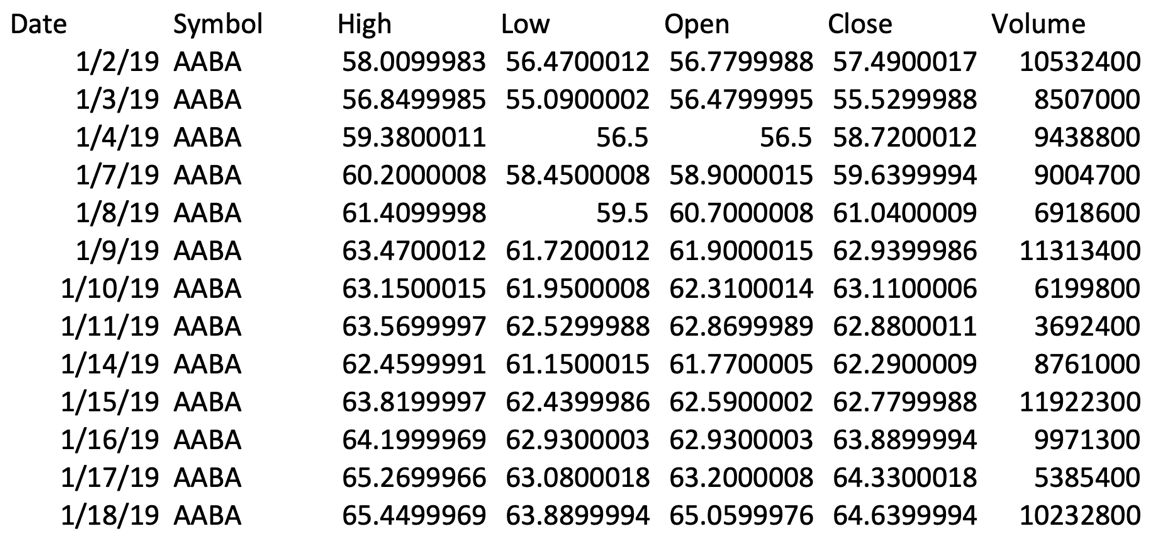
\includegraphics[width=3.5in]{Images/raw_stock_data.png}
	\caption{Slice of raw data obtained from Yahoo daily stock data via Python script.}
	\label{fig:raw_data}
\end{figure}

\subsection{Data Models}

After obtaining sufficient stock exchange data, our next task was to create data models for both relational and graph database systems. These models served to organize the structure of our data for each DBMS, which was necessary before beginning to insert data into the databases. 

\subsubsection{MySQL} 

The first data model we created was an Entity-Relational diagram as depicted in Fig. \ref{fig:mysql_model}, in order to format our data for a MySQL database. Tables were created for the daily input of data collected for each exchange, Amex, Nasdaq, and NYSE. Separate tables were created for calculations, Symbol, Open, Low, High, Close, and Volume. 

Tables were created with the properties listed in Table \ref{tab:daily_data}. Ticker symbols are limited to a six character maximum to alleviate any unused space. Price data for High, Low, Open, Close are all decimal values with eighteen digits and four decimal places. This allows for maximization of space and allocates enough decimal space to keep track of minute changes in lower valued securities which trade in one thousandth of a penny.  

Exchange is comprised of a \texttt{varchar} with six characters since our largest exchange value is Nasdaq which is made up of six characters. The ID and primary key for the tables is an integer with eleven characters. This maximizes the scalability of the relational database model by streamlining the amount of data which has to be collected and then processed.  

To keep the application lean, the data model is also streamlined and very lean to allow for maximum performance. The first set of tables have no relationships between them. These tables are used to house the bulk of daily data, then the data is transferred to the relational tables listed in Table \ref{tab:relational_data}. The Daily data tables are used for posterity of data collection and are not used for any calculation purposes. 

\begin{figure}
	\centering
	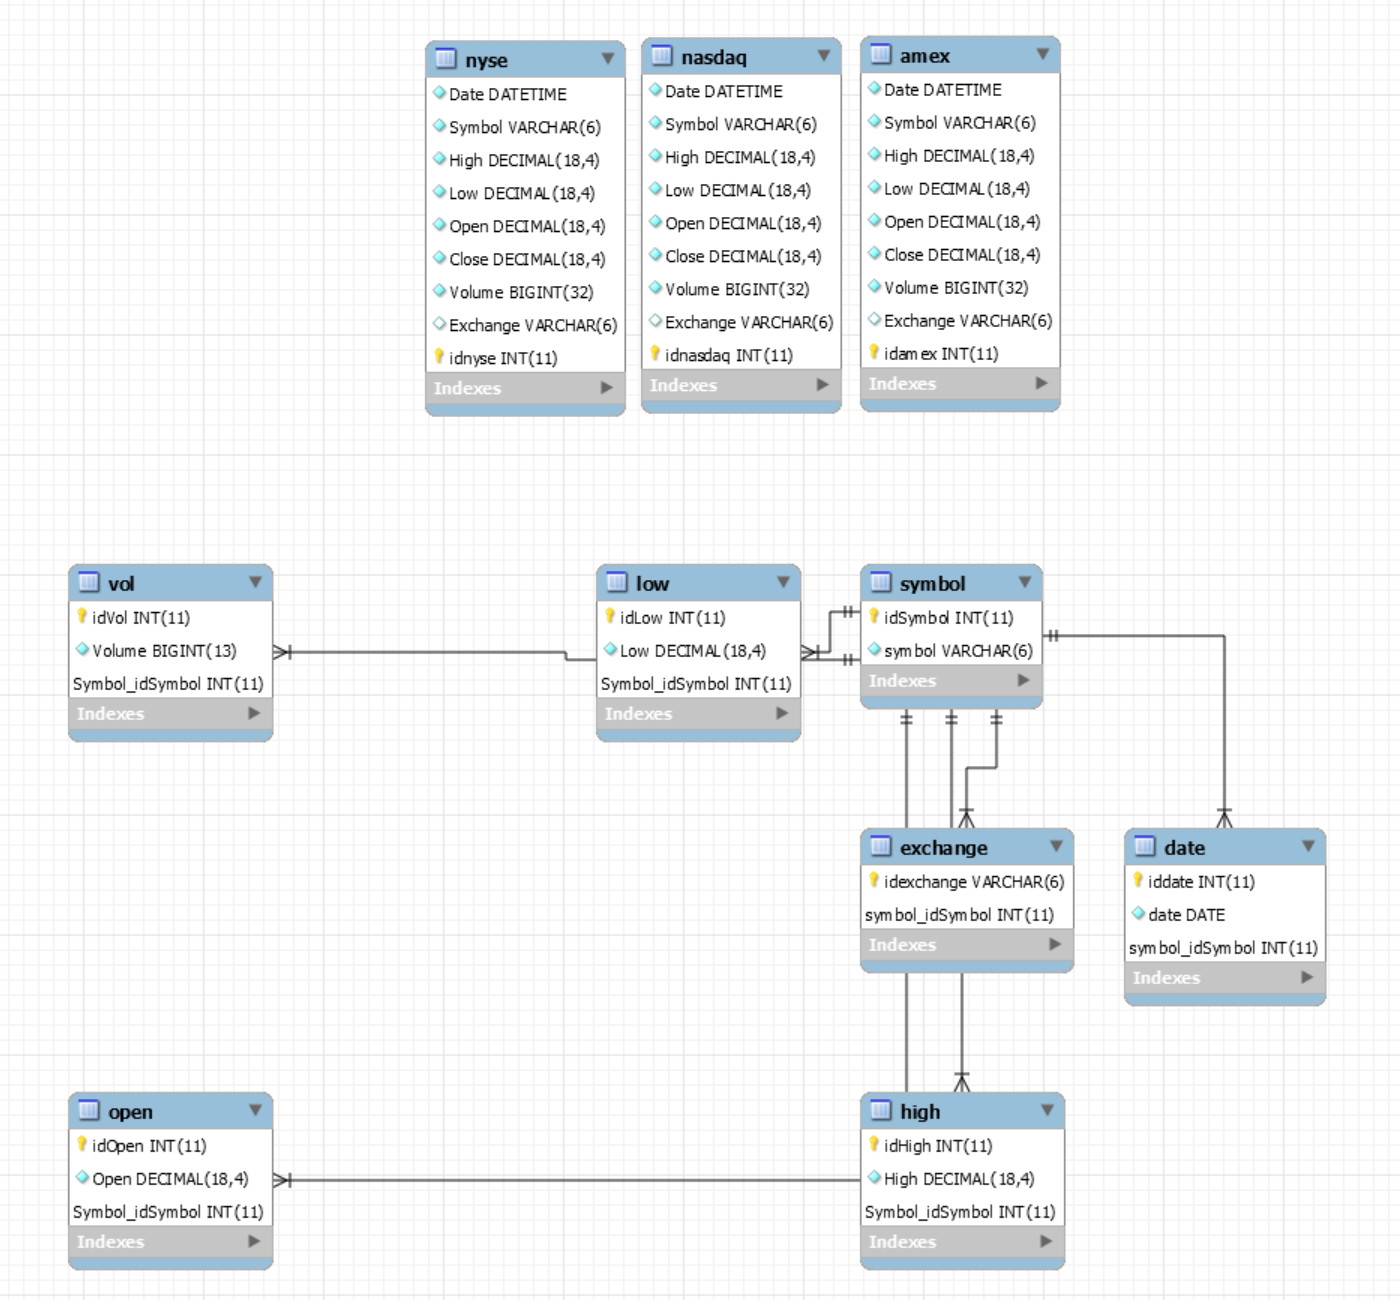
\includegraphics[width=3.5in]{Images/mysql_data_model.png}
	\caption{Data model for MySQL, created in MySQL Workbench.}
	\label{fig:mysql_model}
\end{figure}

\begin{table}
	\centering
	\caption{Relational Database Daily Data Tables}
	\label{tab:daily_data}
\begin{tabular}{ll} \hline \hline
\textbf{Table Name} & \textbf{Properties} \\ \hline
AMEX & Date (Datetime) \\
 & Symbol (VarChar(6)) \\ 
 & High (Decimal(18,4)) \\
 & Low (Decimal(18,4)) \\
 & Open (Decimal(18,4)) \\
 & Close (Decimal(18,4)) \\
 & Volume BigInt(32) \\
 & Exchange VarChar(6) \\
 & IdAmex Int(11) \\ \hline
NASDAQ & Date (Datetime) \\
 & Symbol (VarChar(6) \\
 & High (Decimal(18,4)) \\
 & Low (Decimal(18,4)) \\
 & Open (Decimal(18,4)) \\
 & Close (Decimal(18,4)) \\
 & Volume BigInt(32) \\
 & Exchange VarChar(6) \\
 & IdNasdaq Int(11) \\ \hline
NYSE & Date (Datetime) \\
 & Symbol (VarChar(6) \\
 & High (Decimal(18,4)) \\
 & Low (Decimal(18,4)) \\
 & Open (Decimal(18,4)) \\
 & Close (Decimal(18,4)) \\
 & Volume BigInt(32) \\
 & Exchange VarChar(6) \\
 & IdNYSE Int(11) \\ \hline \hline
\end{tabular}
\end{table}

The second set of tables house the daily information for each of the symbols. The tables are separated into the values listed for each symbol as they are in the daily tables---Symbol, High, Low, Open, Close, Volume, and Exchange. This allows us to collect the specific data and alleviate as much redundancy as possible for calculation. While the daily tables has all daily data and is kept for posterity purposes, the symbol data tables have relationships defined as listed in Table \ref{tab:relational_data}. There are one to many relationships for each of the tables and symbol. Since symbol is the central point of the database, each subsequent table is a subset of data for the symbol. Each property of the table is the same as the Daily tables, with the exception of Volume, which is reduced to a thirteen-character limit as a big integer. This reduces additional memory space required to house the value during calculation time helping to speed up the process. 

\begin{table}
	\centering
	\caption{Relational Database Symbol Data Tables}
	\label{tab:relational_data}
\begin{tabular}{lll} \hline \hline
\textbf{Table} & \textbf{Properties} & \textbf{Relationships} \\ \hline
Symbol & IDSymbol Int(11) & Date: 1:M \\
& Symbol VarChar(6) & High: 1:M \\ 
& & Low: 1:M \\ 
& & Open: 1:M \\
& & Close: 1:M \\
& & Volume: 1:M \\ 
& & Exchange: 1:M \\ \hline
Date & IDDate Int(11) & Symbol\_IDSymbol \\
& Date (DATE) & \\ \hline
High & IDHigh Int(11) & Symbol\_IDSymbol \\
& High Decimal(18,4) & \\ \hline
Low & IDLow Int(11) & Symbol\_IDSymbol \\
& Low Decimal(18,4) & \\ \hline
Open & IDOpen Int(11) & Symbol\_IDSymbol \\
& Open Decimal(18,4) & \\ \hline
Close & IDClose Int(11) & Symbol\_IDSymbol \\
& Close Decimal(18,4) & \\ \hline
Volume & IDVolume Int(11) & Symbol\_IDSymbol \\
& Volume BigInt(13) & \\ \hline
Exchange & IDExchange Int(11) & Symbol\_IDSymbol \\ \hline \hline
\end{tabular}
\end{table}

\subsubsection{Neo4j}

As mentioned before, the four essential data constructs for Neo4j are nodes, labels, relationships, and properties. Working in this context requires a very different mindset from MySQL and the relational model. When creating a data model for Neo4j, we decided to begin from scratch and not let the MySQL model influence the graph database structure. Because we knew that our queries would involve traversing through nodes based on dates, we chose to create individual nodes for each date, and connect sequential days. In this way, the model essentially centers around the dates, which can be iterated through easily.  

In addition, connected to each date are the stock symbols that we have data for; connected to each symbol are the attributes for that day and symbol, including high, low, open, close, volume, and exchange. We chose to break all of these attributes into their own nodes rather than retain them as properties on the symbol node, because Neo4j can make checks against nodes more efficiently than against properties \cite{neo4j-book}. Fig. \ref{fig:neo4j_model} shows the Neo4j graph with only a few days and symbols, so that the relationships can be clearly seen. Fig. \ref{fig:neo4j_gen_model} represents the generalized data model, indicating the relationships and labels present in the database. 

\begin{figure}
	\centering
	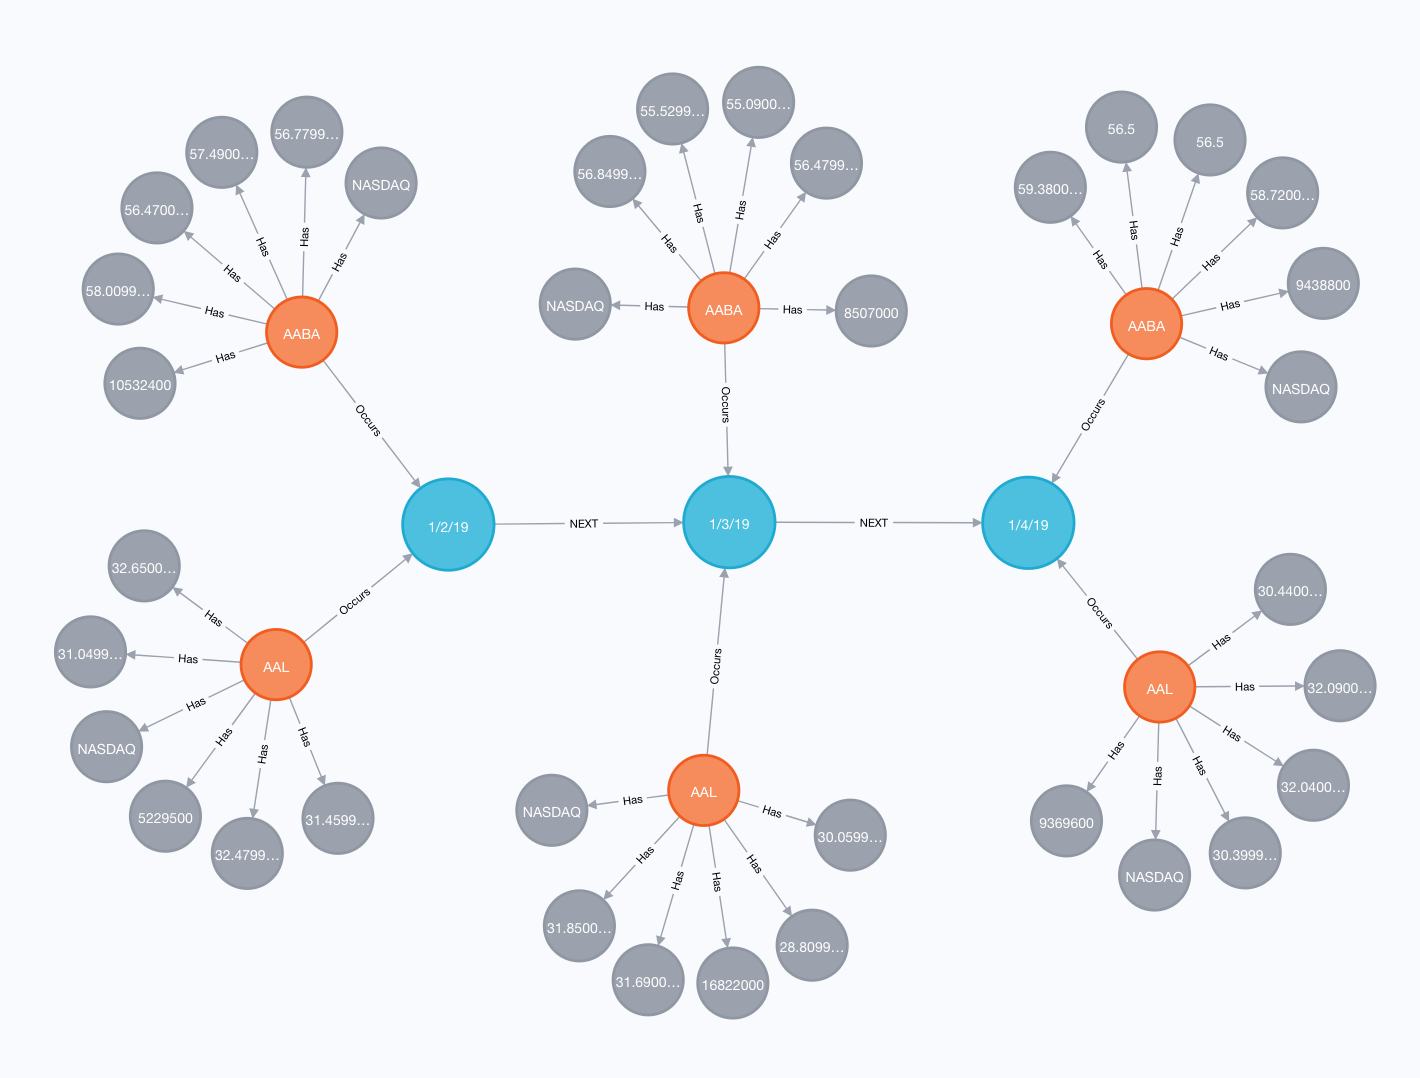
\includegraphics[width=3.5in]{Images/neo4j_data_model.png}
	\caption{Representation of sample data in Neo4j}
	\label{fig:neo4j_model}
\end{figure}

\begin{figure}
	\centering
	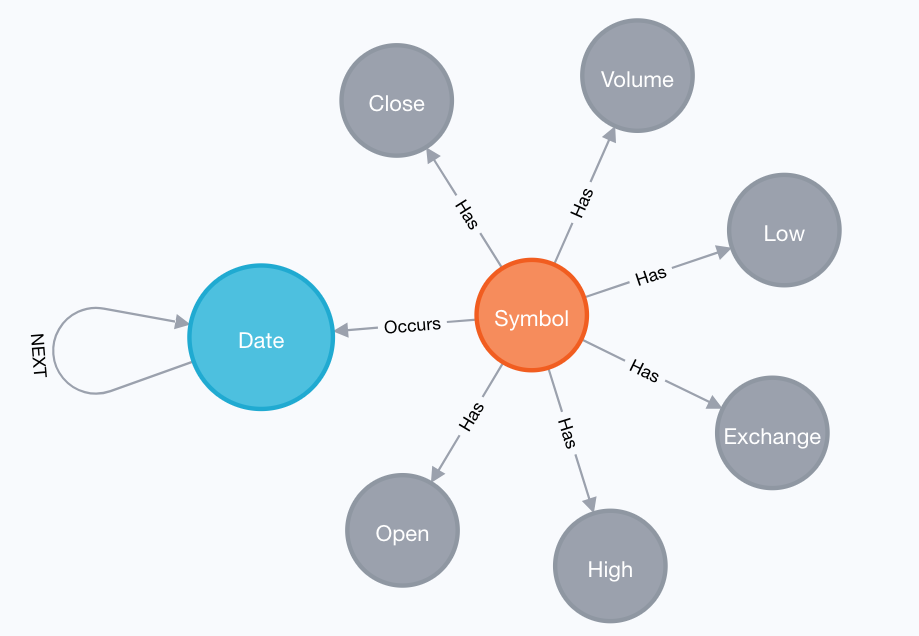
\includegraphics[width=3.5in]{Images/neo4j_general_model.png}
	\caption{Generalized data model for Neo4j}
	\label{fig:neo4j_gen_model}
\end{figure}

\subsection{VIR Calculation}

In order to make a Volatility Index calculation, we needed a minimum of 22 days' worth of data. We have a few more days than this available, but we have begun by calculating single VIR statistics for a given company on a certain day. 

\subsubsection{MySQL}

Not yet completed.

\subsubsection{Neo4j}

We were able to make the VIR computation with our Neo4j database using the query language Cypher. As seen in Equation \ref{eq:vir}, the first value to be calculated is the highest close over those 22 days. The following Cypher query obtains this value.
\begin{verbatim}
match (d:Date)-[:Occurs]-(s:Symbol)
      -[:Has]-(p:Close)  
where s.name="ACU" and d.val>="2019-01-02" 
      and d.val<="2019-01-31" 
return max(p.val) 
\end{verbatim} 

In this query, pattern-matching is performed on the nodes with Date, Symbol, and Close labels. The \texttt{where} clause filters the desired symbol and sequence of days, and the \texttt{return} statement aggregates the Close numbers and finds the maximum value. We performed similar queries to find the highest High over those days and the current Low for the final day in the sequence. Plugging these values into Equation \ref{eq:vir}, we obtained the (rounded) result $\text{VIR} = \frac{17.02 - 16.71}{17.97}\cdot 100 = 1.725\%$ for the company with the ticker symbol ACU (that is, Acme United Corporation) on January 31st, 2019.  

Our next step is to programmatically calculate the VIR for a given symbol over a sequence of days, rather than run individual queries manually. We can then create our own VIR graphs similar to Fig. \ref{fig:vir_example} if desired, as well as evaluate the performance of such queries that make bulk calculations. 

\subsection{Performance Tests}

Once we write scripts for both MySQL and Neo4j to be able to perform bulk queries, we will run these scripts and record performance metrics using Paul’s Microsoft Performance Monitor. Those metrics include CPU, RAM, and disk performance statistics. In this section we will describe the different queries that we ran to compare. (Note: We are waiting to write these bulk queries until we obtain additional historical data. The Yahoo API has recently changed its allowances, and we have not yet found a reliable/efficient workaround.)

\section{Results}

Here we will include all the performance statistics obtained from our performance tests described above. Those statistics include the OS metrics of CPU, RAM, and disk performance, as well as DBMS internal statistics such as execution time. (For reference, the Cypher queries that obtained the VIR on a single day, as described earlier, completed in 108 ms.) 

\section{Analysis of Results}

Here we will provide commentary on our complete results. We will also include a suitability analysis, i.e. describe and compare how we felt the two database systems accommodated our stock exchange data.

\section{Future Work}

Here we will address any aspects of the research that we did not complete, or interesting variations of the problem that could be investigated. 

\section{Conclusions}

We are waiting to write our final conclusions until all of our analysis is complete. 

\bibliographystyle{IEEEtran}
\bibliography{Bibliography}

\end{document}
